
\section{CPN Tools and Applications}

The construction and analysis of CPN models have been supported by two
generations of graphical computer tools. The first generation was the
Design/CPN tool \cite{jensen:cpnmanual} which was developed starting
in the mid 80'es at Meta Software Corp. and later by the CPN Group at
the Aarhus University. This was followed by CPN Tools
\cite{cpntoolsweb} that has been developed since 2000 first by the CPN
Group at Aarhus University and since 2009? by the XX group at the
Technical University of Eindhoven. CPN Tools supports the editing and
construction of CPN models, interactive and automatic simulation,
state space-based model checking, and simulation-based performance
analysis. Both Design/CPN and CPN Tools has been widely distributed
tools and they have been applied for modelling and validation in a
broad range of application domains. Below we provide some pointer to
some selected applications within typical application domains. A more
comprehensive list of example applications and domains can be found
via \cite{cpnuse}.

\begin{figure*}[b]
\centering
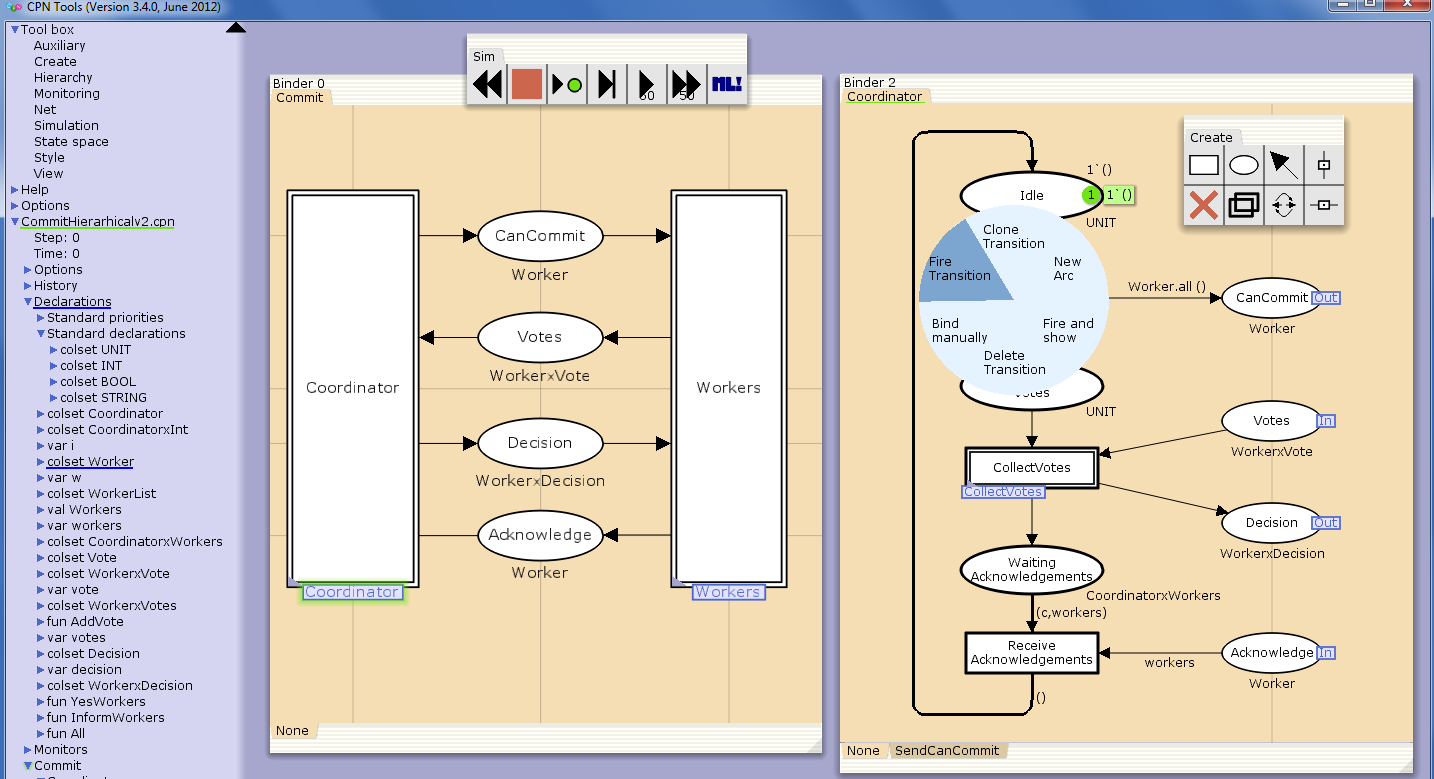
\includegraphics[width=\textwidth]{figures/cpntools.png}
\caption{Two-phase Commit Protocol in CPN Tools}
\label{fig:cpntools}
\end{figure*}


Figure~\ref{fig:cpntools} provides a screenshot of CPN Tools. The user
of CPN Tools works directly with the graphical representation of the
CPN model. The graphical user interface (GUI) of CPN Tools has no
conventional menu bars and pull-down menus, but is based on
interaction techniques, such as \concept{tool palettes} and
\concept{marking menus}. The rectangular area to the left is an
\concept{index}. It includes the \figitem{Tool box}, which is
available for the user to manipulate the declarations and modules that
constitute the CPN model. The \figitem{Tool box} includes tools for
creating, copying, and cloning the basic elements of CP-nets. It also
contains a wide selection of tools to manipulate the graphical layout
and the appearance of the objects in the CPN model. The latter set of
tools is very important in order to be able to create readable and
graphically appealing CPN models. The remaining part of the screen is
the \concept{workspace}, which in this case contains four
\concept{binders} (the rectangular windows) and a circular pop-up
menu.

Each binder holds a number of items which can be accessed by clicking
the tabs at the top of the binder (only one item is visible at a
time). There are two kinds of binders. One kind contains the elements
of the CPN model, i.e., the modules and declarations. The other kind
contains the tools which the user applies to construct and manipulate
CPN models. The tools in a tool palette can be picked up with the
mouse cursor and applied. In the example shown, one binder contains
three modules named \figitem{Protocol}, \figitem{Sender}, and
\figitem{Receiver}, while another binder contains a single module,
named \figitem{Network}, together with the declaration of the colour
set \smlcode{NOxDATA}. The two remaining binders contain four
different tool palettes to \figitem{Create} elements, change their
\figitem{Style}, perform \figitem{Simulations}, and construct
\figitem{State spaces}.

Items can be dragged from the index to the binders, and from one
binder to another binder of the same kind. It is possible to position
the same item in two different binders, for example, to view a module
using two different zoom factors. A circular marking menu has been
popped up on top of the bottom left binder. Marking menus are
contextual menus that make it possible to select among the operations
possible on a given object. In the case of
Fig.~\ref{fig:cpntoolssnapshot}, the marking menu gives the operations
that can be performed on a port place object.

% syntax check and code generation

CPN Tools performs syntax and type checking, and error messages are
provided to the user in a contextual manner next to the object causing
the error. The syntax check and code generation are incremental and
are performed in parallel with editing. This means that it is possible
to execute parts of a CPN model even if the model is not complete, and
that when parts of a CPN model are modified, a syntax check and code
generation are performed only on the elements that depend on the parts
that were modified. The main outcome of the code generation step is
the \concept{simulation code}. The simulation code contains the
functions for inferring the set of enabled events in a given state of
the CPN model, and for computing the state resulting from the
occurrence (execution) of an enabled event in a given state.

% simulation

CPN Tools supports two types of simulation: interactive and
automatic. In an interactive simulation, the user is in complete
control and determines the individual steps in the simulation, by
selecting between the enabled events in the current state. CPN Tools
shows the effect of executing a selected step in the graphical
representation of the CPN model. In an automatic simulation the user
specifies the number of steps that are to be executed and/or sets a
number of stop criteria and breakpoints. The simulator then
automatically executes the model without user interaction by making
random choices between the enabled events in the states
encountered. Only the resulting state is shown in the GUI. A
\concept{simulation report} can be saved, containing a specification
of the steps that occurred during an automatic simulation. The
simulator of CPN Tools exploits a number of advanced data structures
for efficient simulation of large hierarchical CPN models. The
simulator exploits the locality property of Petri nets to ensure that
the number of steps executed per second in a simulation is independent
of the size of the CPN model. This guarantees that simulation scales
to large CPN models.

TALK/REFER TO THINGS ABOUT INDUSTRIAL APPLICATIONS IN THE END

\paragraph{Embedded Systems} Dalcotech or B and O

\paragraph{Process Scheduling} COAST

\paragraph{Internet Protocols} ERDP

\paragraph{Mobile Phone Software} NOKIA

\paragraph{Capacity Planning} HP

